\section{Task II : Key Events}
\subsection{Key Events}
\subsubsection{Calculation Methods}
To identify key events, we will use the proportion of medals from these events among the whole medal tally as a main factor.

\begin{figure}[htbp]
    \centering
    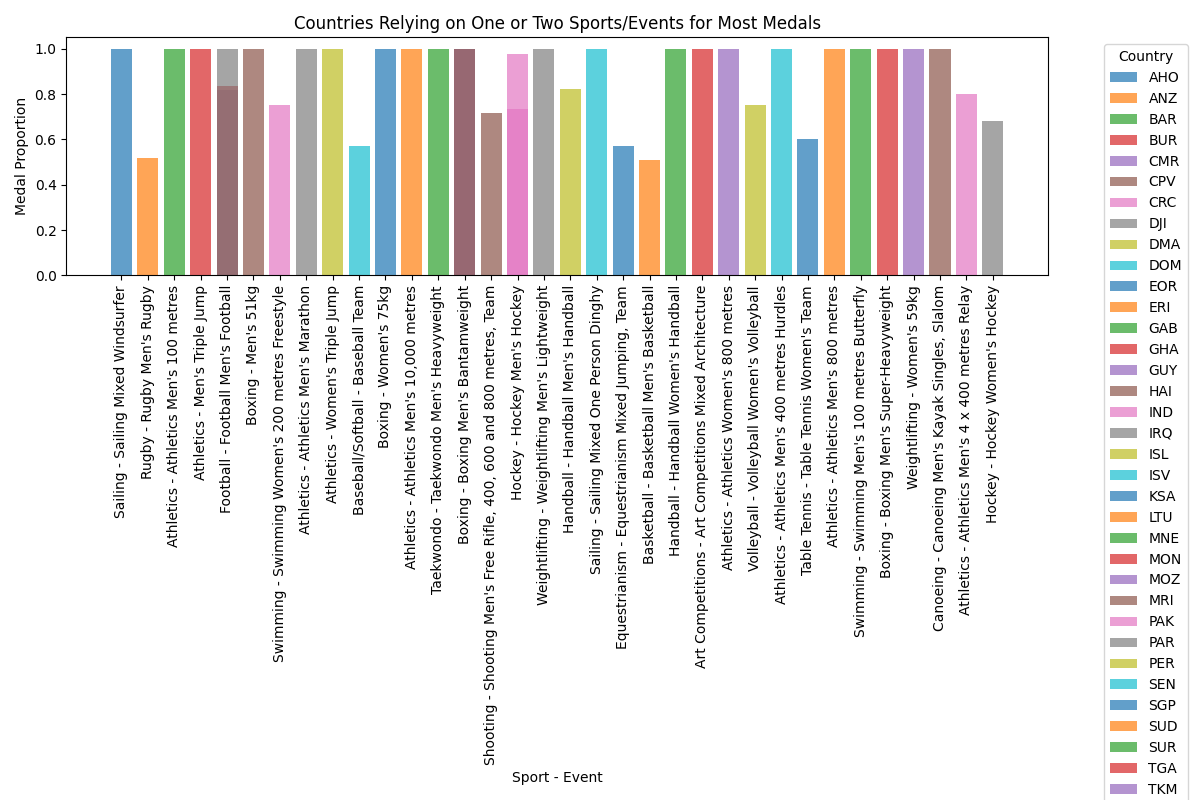
\includegraphics[width=1.1\textwidth]{./figures/Key_event.png}
    \caption{ Countries with biased medal distribution}
    \label{fig:Key_event}
\end{figure}

From this graph, we can see that many countries rely on one or two sports/events for their medal tally. This can be inspiring for the countries' Olympics committees.
